\subsection{Moduł pacjenta}



\begin{itemize}
	\item Pacjent w celu korzystania z usług placówki musi posiadać konto w systemie. Zaimplementowane funkcjonalności w oparciu o wymagania od 27 do 32 umożliwiają rejestrację, logowanie, resetowanie i zmianę hasła, zmianę adresu email oraz wylogowanie z systemu.

\vspace{0,5cm}
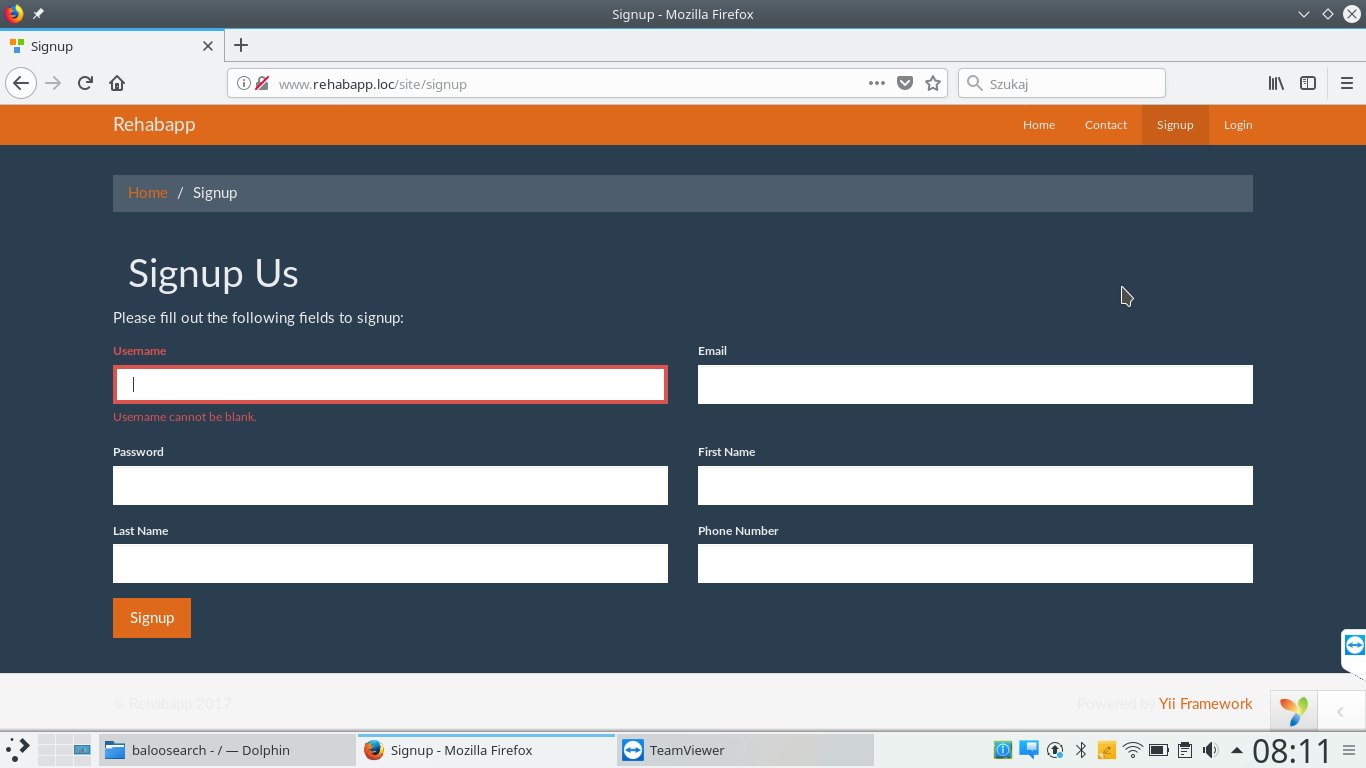
\includegraphics[scale=0.4]{obraz/17.png}
%\begin{center}{\scriptsize Rysunek 1: Diagram przypadków użycia.}\end{center}
\vspace{0,5cm}

\vspace{0,5cm}
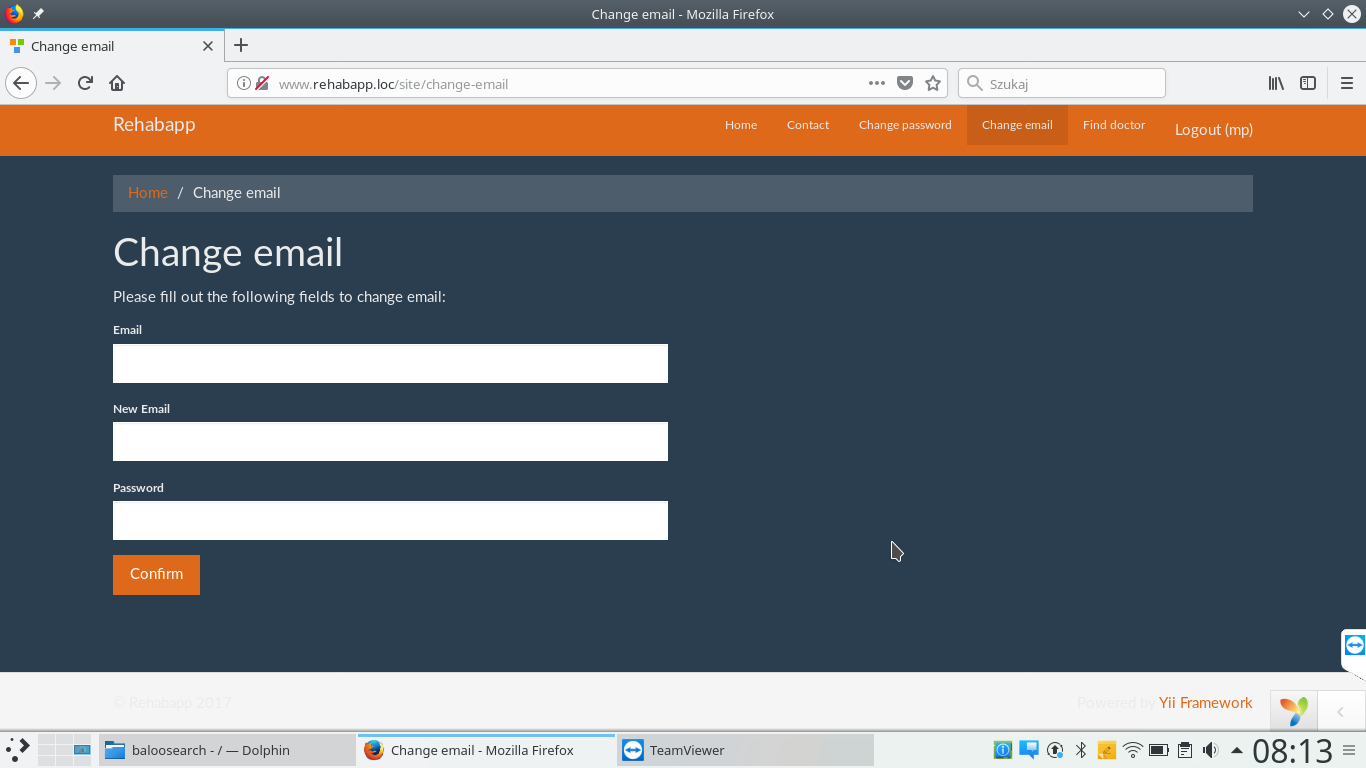
\includegraphics[scale=0.4]{obraz/19.png}
%\begin{center}{\scriptsize Rysunek 1: Diagram przypadków użycia.}\end{center}
\vspace{0,5cm}

\vspace{0,5cm}
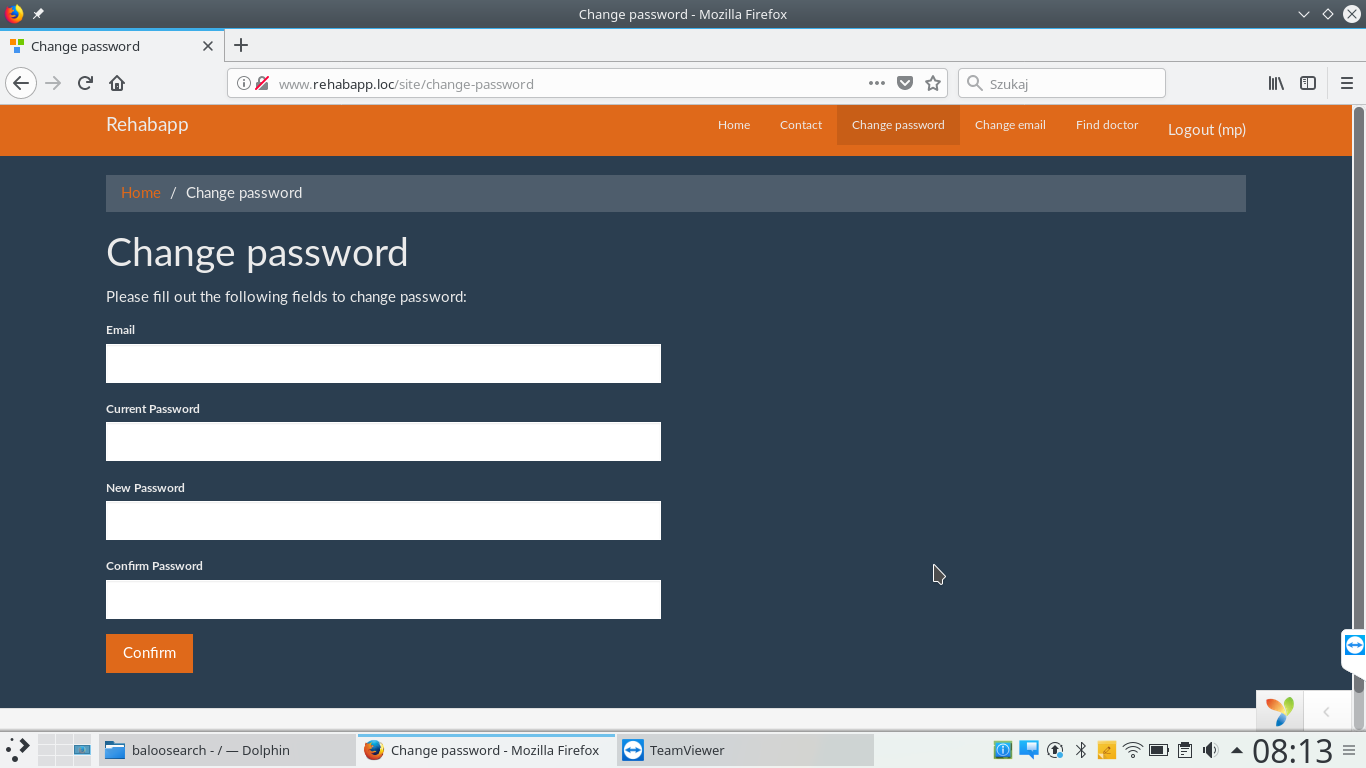
\includegraphics[scale=0.4]{obraz/20.png}
%\begin{center}{\scriptsize Rysunek 1: Diagram przypadków użycia.}\end{center}
\vspace{0,5cm}

	\item Pacjent ma możliwość wyszukiwania lekarzy i wyświetlania ich profili.
	
\vspace{0,5cm}
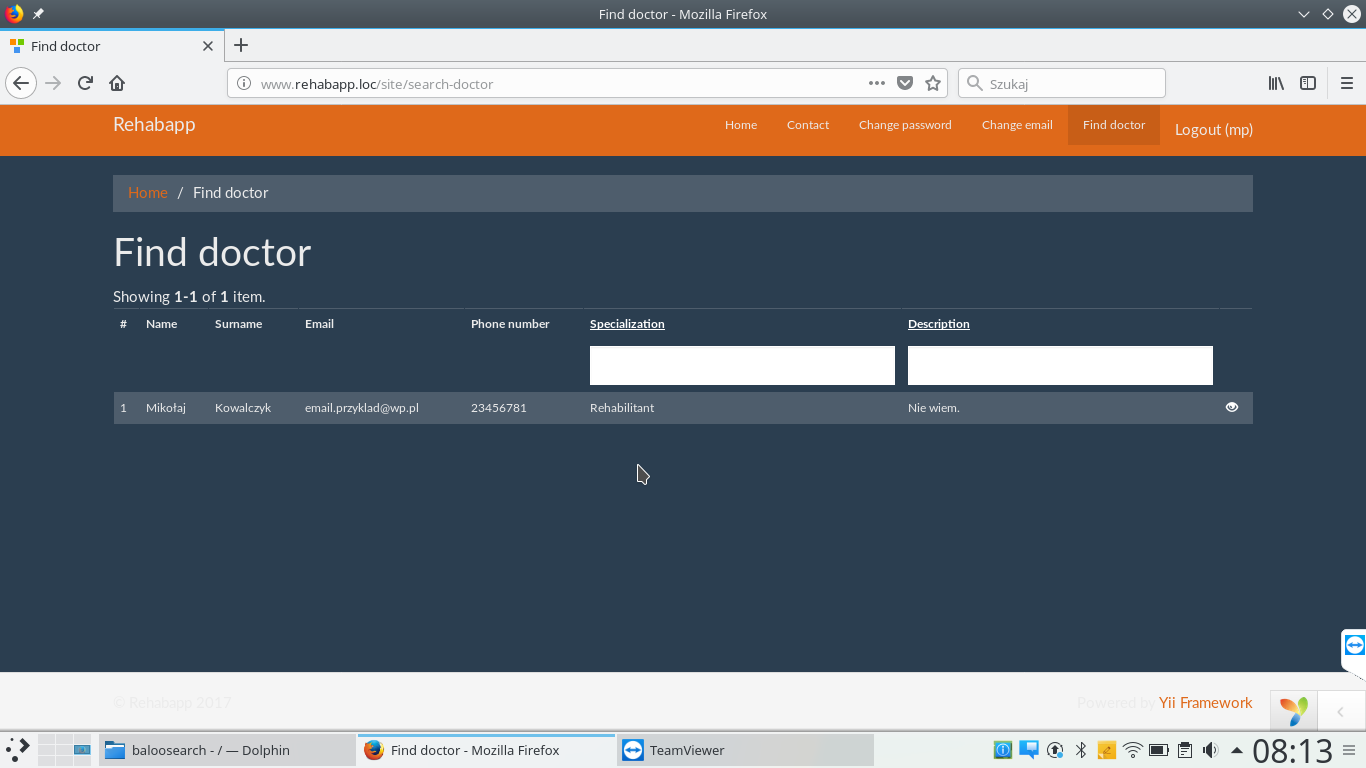
\includegraphics[scale=0.4]{obraz/18.png}
%\begin{center}{\scriptsize Rysunek 1: Diagram przypadków użycia.}\end{center}
\vspace{0,5cm}

\vspace{0,5cm}
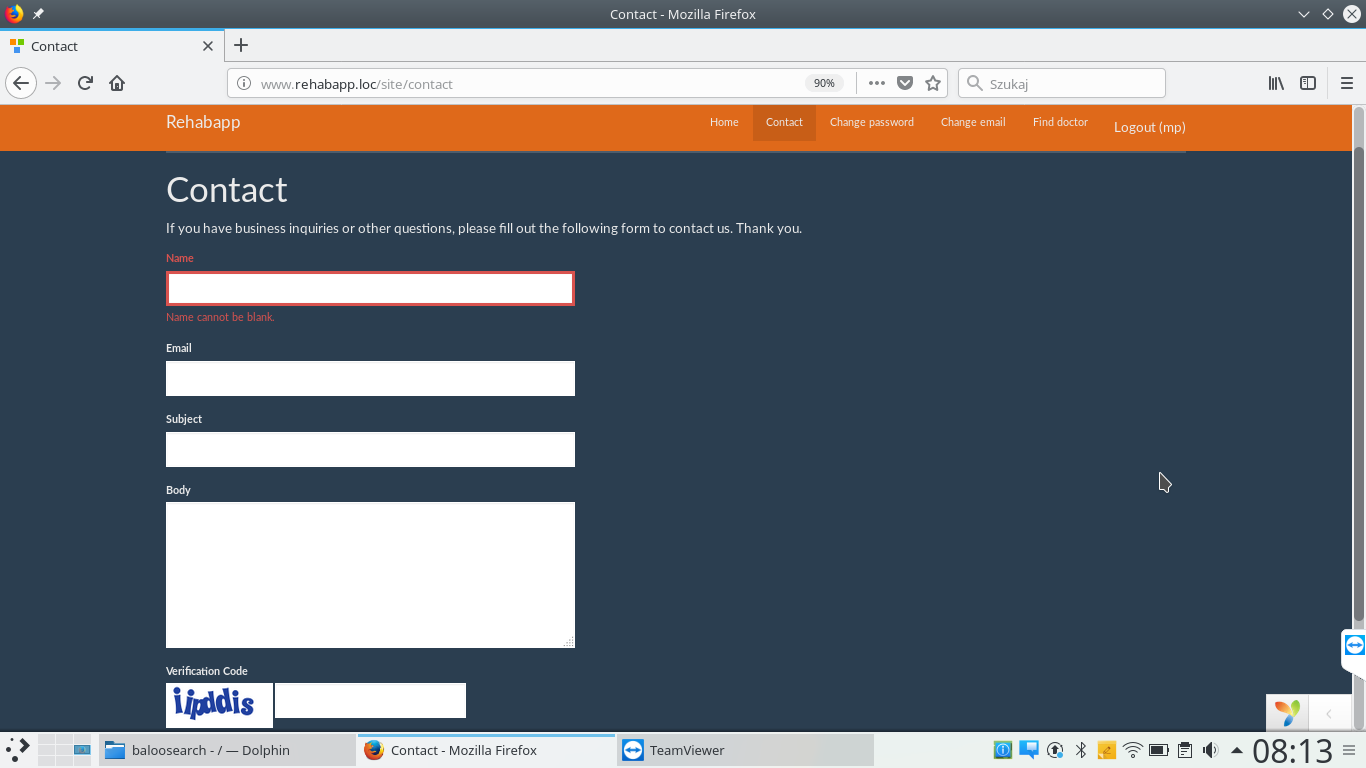
\includegraphics[scale=0.4]{obraz/21.png}
%\begin{center}{\scriptsize Rysunek 1: Diagram przypadków użycia.}\end{center}
\vspace{0,5cm}


\end{itemize}